\documentclass[a4paper,10pt]{article}
\usepackage[utf8]{inputenc}
\usepackage{graphicx} % Allows including images
\usepackage{amsmath} %fancy math commands
\usepackage{amssymb} %math symbols
\usepackage{booktabs} % Allows the use of \toprule, \midrule and \bottomrule in tables
\usepackage{multicol} %two columns single page
\usepackage{blindtext} %sample text
\usepackage{threeparttable} %tables with annotations
\usepackage{verbatim} %allows commenting
\usepackage{setspace} %allows changing line spacing and turns off double spacing in tables
\usepackage{mwe} % new package from Martin scharrer
\usepackage{caption} % specific captions for minipage
\usepackage[section]{placeins} % keep figures inside sections
%%%%%%%%%%%%%%%%%%%%%%%%%%% Unicode symbols such as smiles %%%%%%%%%%%%%%%%%%%%%%%%%%%%%%%%%%
\usepackage{wasysym}
%opening
\title{Report on CPD based Coupled Cluster}
\author{Roman Schutski}

\begin{document}

\maketitle

\section{Description}

As was shown earlier, Coupled Cluster can be solved approximately by imposing 
some tensor decomposition with low number of parameters on cluster amplitudes. By combining 
this with an approximation of the Hamiltonian and the "energy denominator" tensors one can 
produce variants of Coupled Cluster theory with low scaling. 
In these notes the results for Canonical Decomposition of amplitudes, RI decomposition
of the two electron integrals and canonical decomposition of energy denominator are 
listed. 
As a reminder, RI and CPD decompositions are defined as

\begin{equation}
V_{ijkl} = \sum_{pq}^{R_{v}} W^{1}_{ijp} \cdot S_{pq} \cdot W^{2}_{qkl}  
\end{equation}

\begin{equation}
T^{2}_{ijab} = \sum_{t}^{R_{t}} X^{1}_{it} \cdot X^{2}_{jt} \cdot X^{3}_{at} \cdot X^{4}_{bt}  
\end{equation}

\begin{figure}[!ht]
\centering
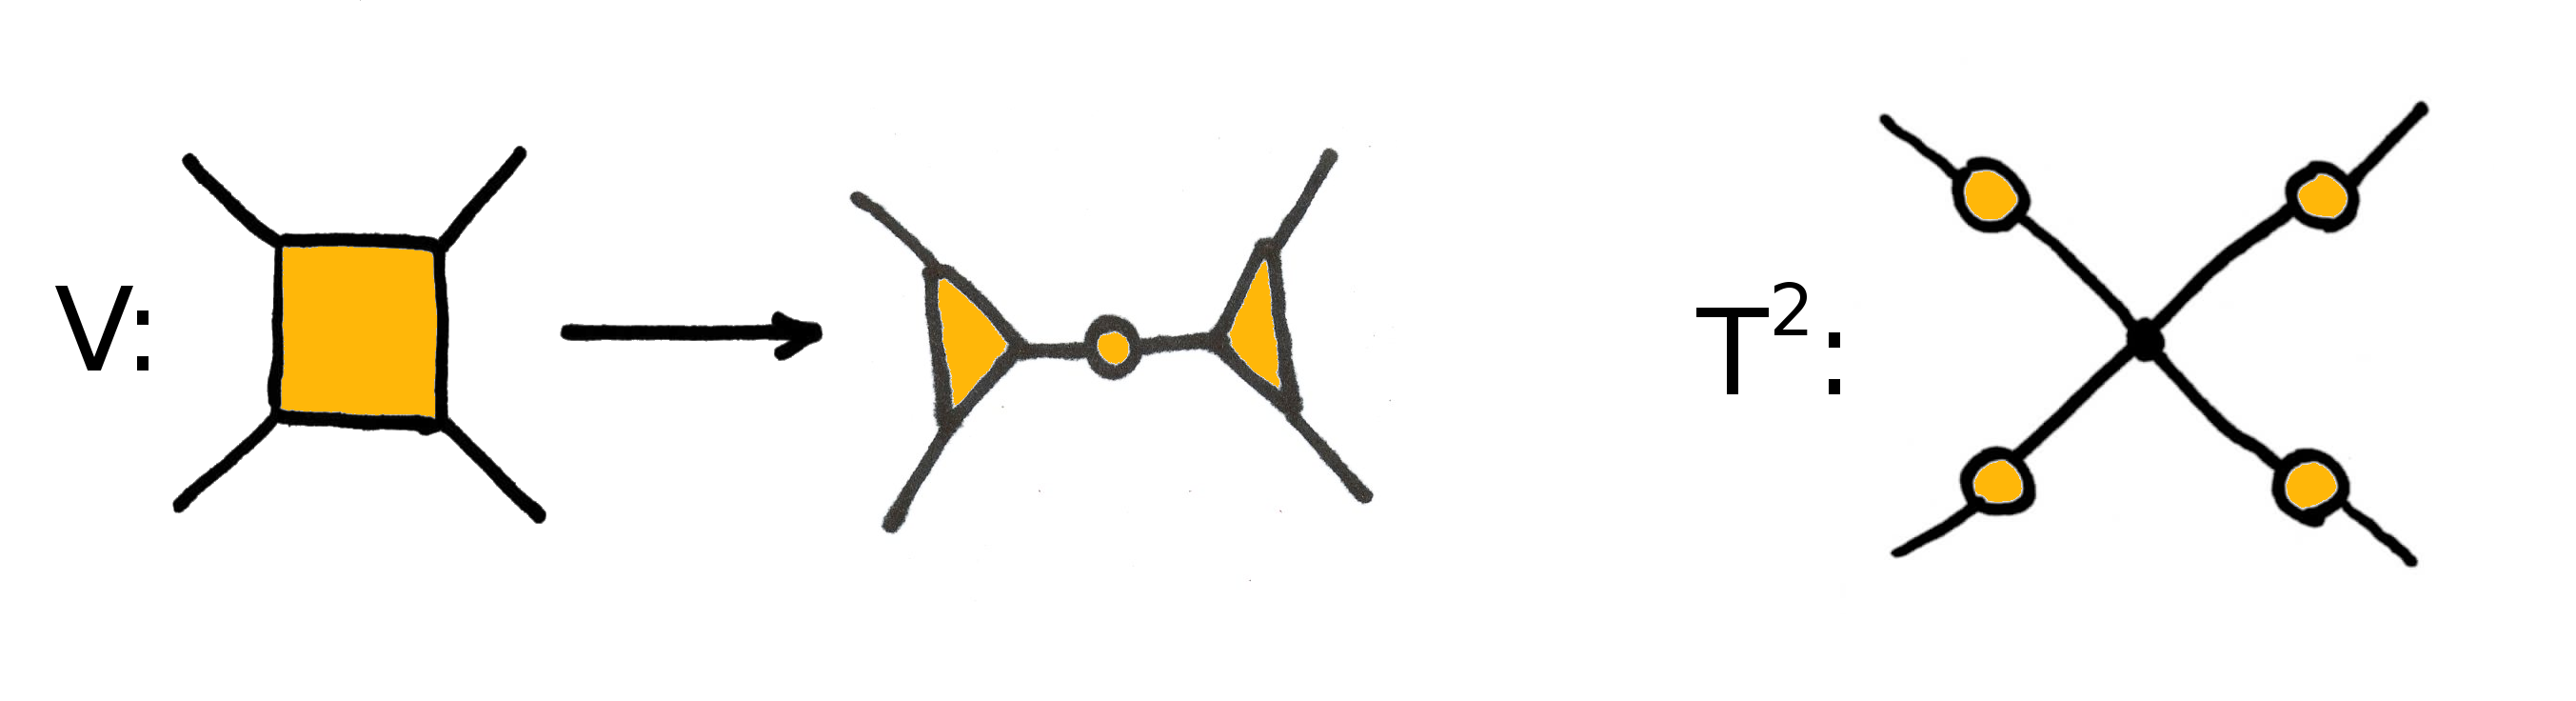
\includegraphics[height=20mm]{graphics/cpd_cc.png}
\end{figure}
 
To estimate the norm of each rank-1 tensor in the CPD,
I sligthly modified CPD decomposition of $T^{2}$ and forced the columns of
$X^{n}$ to have unit norms. The normalized decomposition is defined as
\begin{equation}
T^{2}_{ijab} = \sum_{t}^{R_{t}} \Lambda_{t} X^{1}_{it} \cdot X^{2}_{jt} \cdot X^{3}_{at} \cdot X^{4}_{bt}  
\end{equation}
where $\Lambda$ is a vector containing weights of the normalized factors. The new decomposition 
is denoted as nCPD, and seems to have almost identical properties to the original one.
All discussed Coupled Cluster codes were derived both for CPD and nCPD decomposed amplitudes.

\section{Approximation properties}
Let us start with the discussion of the RCCSD-CPD. Energy behavior versus the rank of CPD for various 
systems is shown below. 
 
\begin{figure}[!htb]
\centering
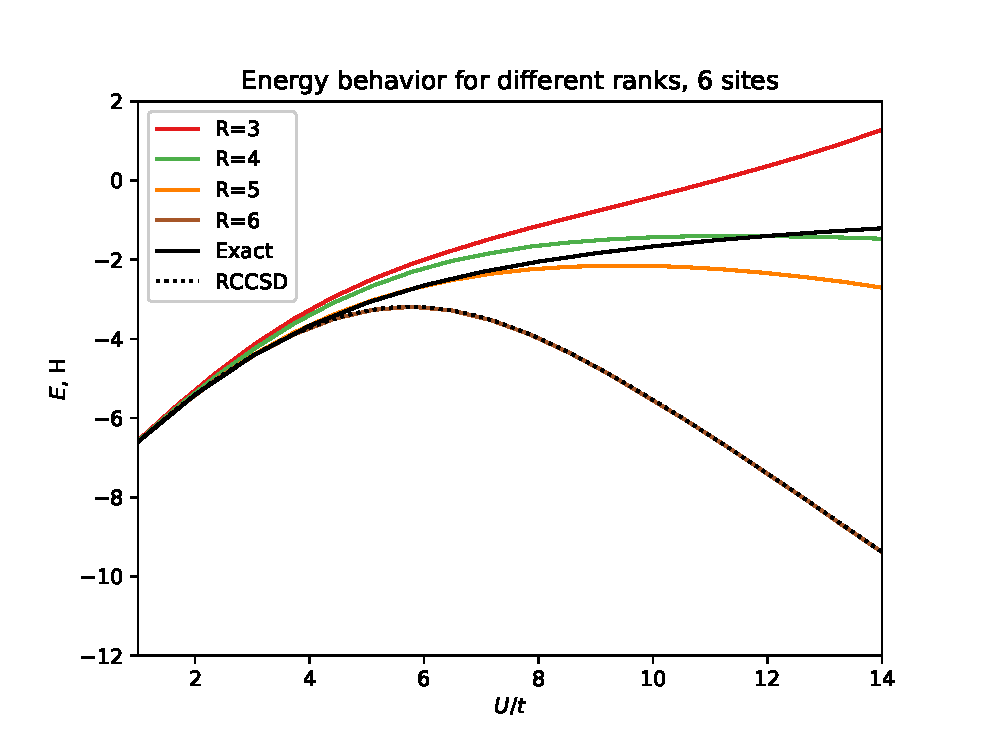
\includegraphics[width=0.9\textwidth]{figures/energy_vs_u_6_sites.eps}
\end{figure}

\begin{figure}[!htb]
\centering
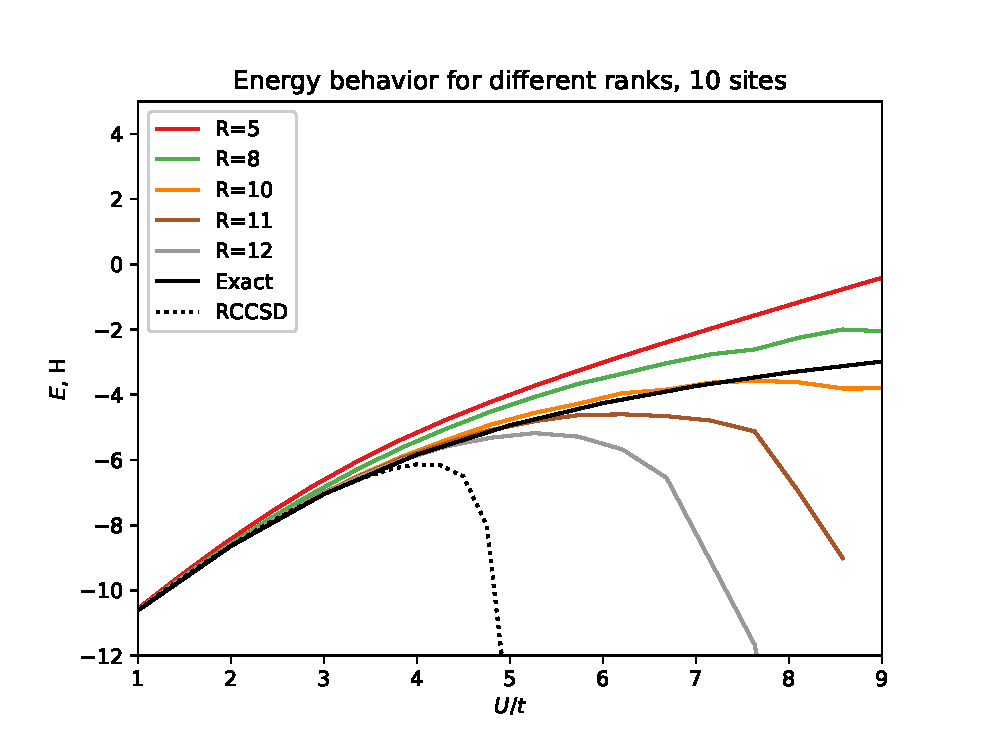
\includegraphics[width=0.9\textwidth]{figures/energy_vs_u_10_sites.eps}
\end{figure}

\begin{figure}[!htb]
\centering
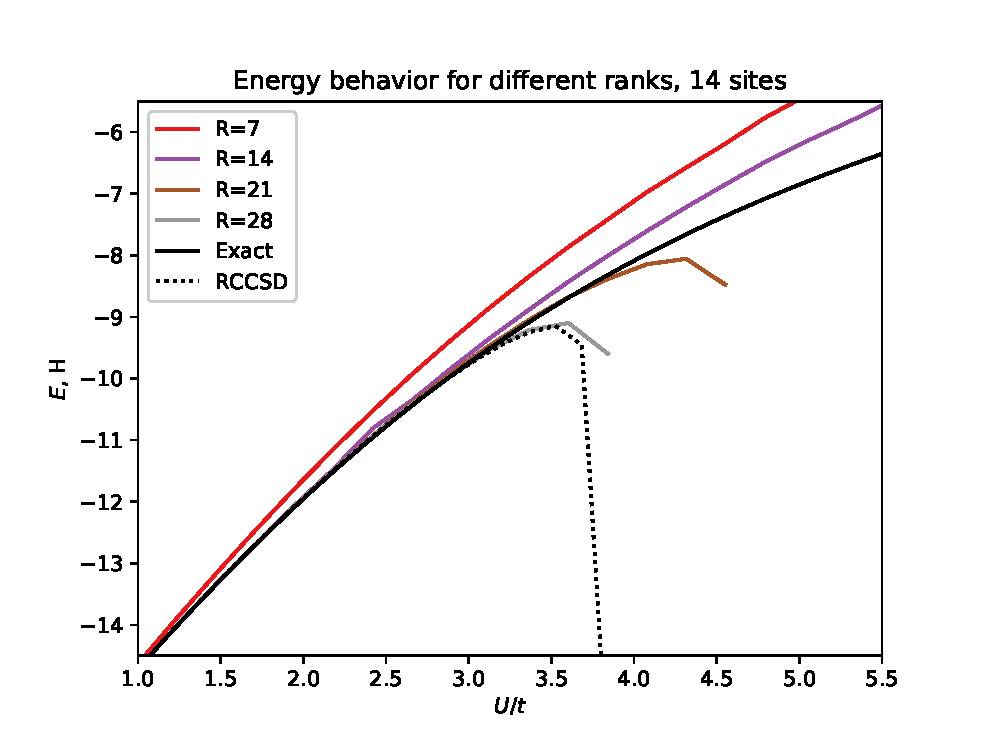
\includegraphics[width=0.9\textwidth]{figures/energy_vs_u_14_sites.eps}
\end{figure}

\begin{figure}[!htb]
\centering
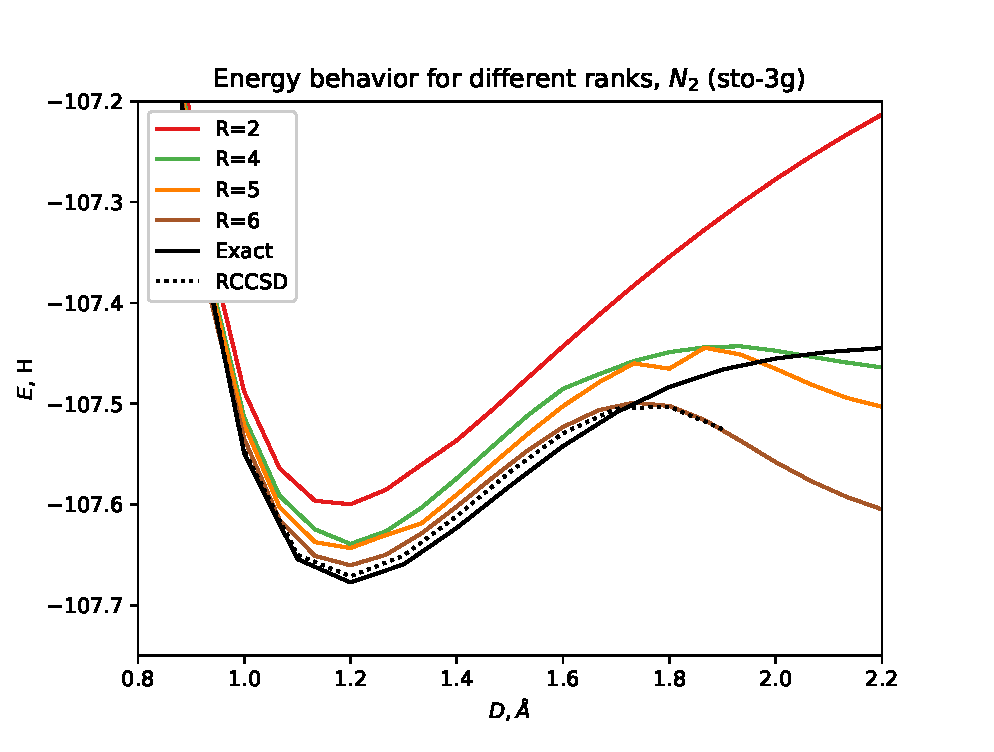
\includegraphics[width=0.9\textwidth]{figures/energy_vs_d_sto-3g.eps}
\end{figure}

\begin{figure}[!htb]
\centering
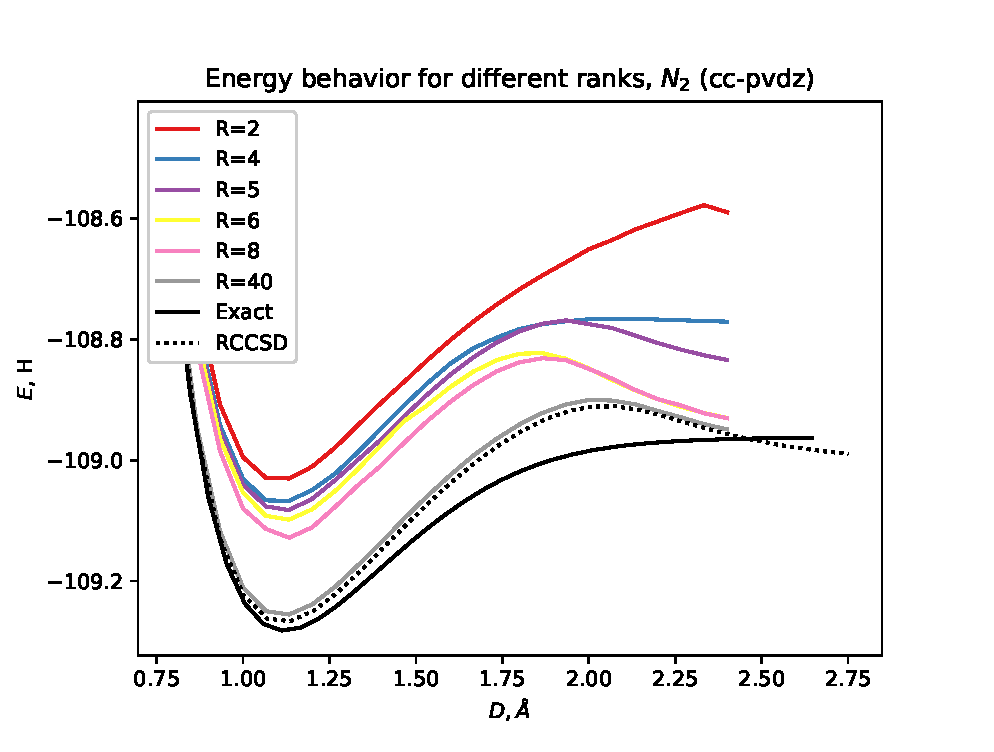
\includegraphics[width=0.9\textwidth]{figures/energy_vs_d_cc-pvdz.eps}
\end{figure}


The performance of the method has distinct features in two regimes: weak and 
strong correlation. In weak correlation regime the errors are small. In strong
correlation regime the difference between approximate and regular Coupled Cluster
may be large, but approximate solutions have better behavior compared to regular ones.

We have to note that the method is not convergent for large ranks at strong correlation.
Normal Coupled Cluster is also non convergent by naive iterations unless damping or 
DIIS is used. I have not found a robust way to do DIIS in the current implementation. 
This aspect needs more thinking and experimentation. Additionally, CC methods with 
decomposed amplitudes may require a lot a iterations to converge.
\section{Weak correlation}
Let us estimate how well the approximation works in the weak correlation case. 

\begin{figure}[!htb]
\centering
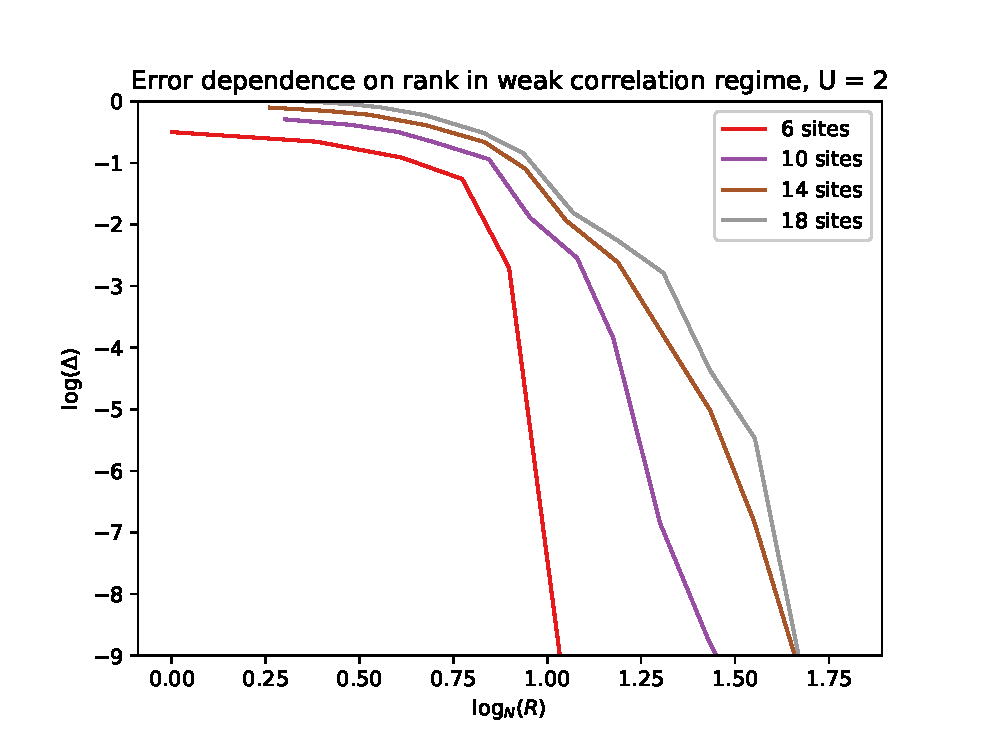
\includegraphics[width=0.9\textwidth]{figures/err_vs_r_u_2_cpd.eps}
\end{figure}

For weak correlation the difference in the energy between RCCSD-CPD and classical RCCSD
decays exponentially with respect to the decomposition rank, which is less than $N^2$. 
We have to note that a fixed $U=2$ does not set an equivalent correlation strength
for tested Hubbard models.

\section{Strong correlation}
It's interesting to note that in strong correlation limit very low rank decompositions 
seem to generate solutions with good physical behavior. Let us look at other 
parameters of Coupled Cluster in this regime. We consider a $10$-site Hubbard with PBC at $U=2$.


\begin{figure}[!htb]
\centering
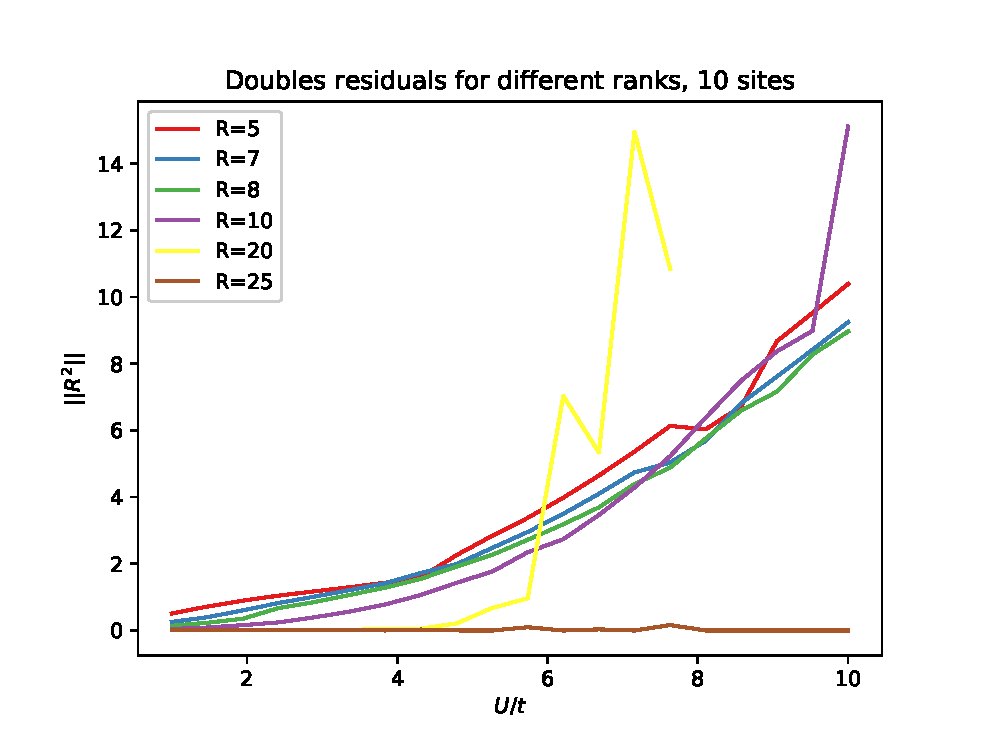
\includegraphics[width=0.9\textwidth]{figures/r2_norms_vs_u_10_sites.eps}
\end{figure}

Decomposed amplitudes are not exact solutions of CC equations. As correlation strength
grows doubles residuals of RCCSD-CPD increase (and equations are getting progressively harder to converge).
As the rank grows those residuals decrease, because decomposed solutions are becoming better
approximations to the conventional CC amplitudes, where all residuals are zero.

$T^{1}$ amplitudes are, however, true solutions to CC equations, because we do not approximate them. 
This results in $T^{1}$ amplitudes becoming non-zero at convergence as they adapt to approximate low-norm $T^{2}$,
while they should be zero for Hubbard models due to symmetry. As the rank of the decomposition increases
$T^{1}$ amplitudes go to their expected values (zero).

\begin{figure}[!htb]
\centering
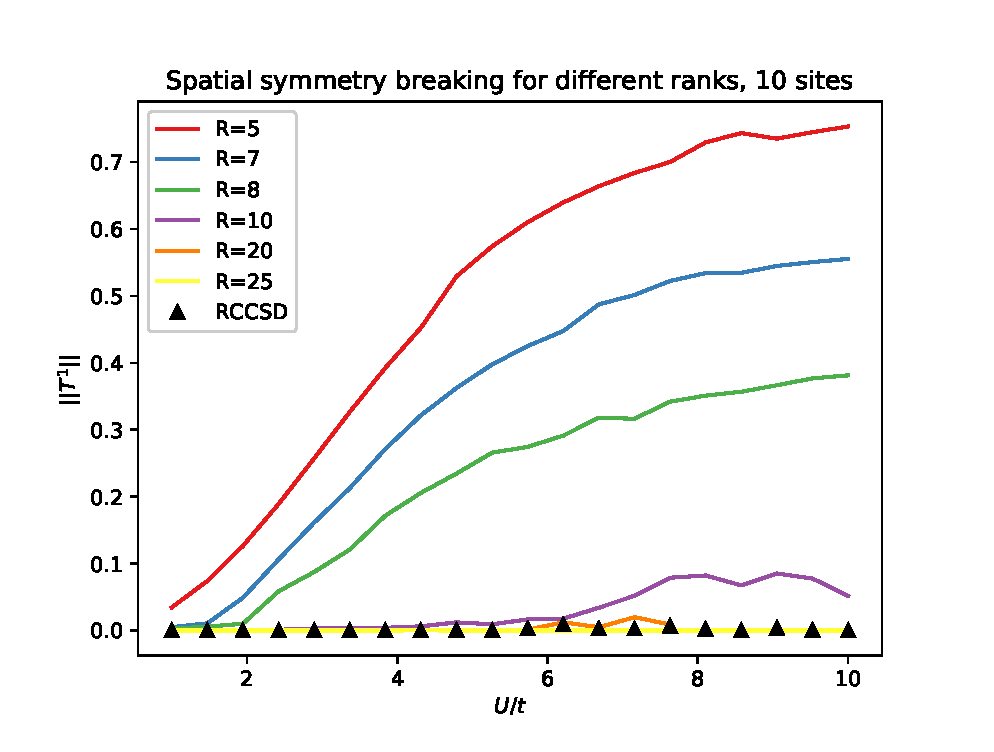
\includegraphics[width=0.9\textwidth]{figures/t1_norms_vs_u_10_sites.eps}
\end{figure}

Let us look at the norm of $T^{2}$.
As was found in PoST and Attenuated-CC works, the cause of the bad performance
of Coupled cluster in strong correlation regime is the growth of higher order
CC amplitudes. It turns out that low rank structure of $T^{2}$ has an effect of 
regularization. As the rank increases, $T^{2}$ amplitudes are getting less regularized 
and approach their conventional values, which are high.

\begin{figure}[!htb]
\centering
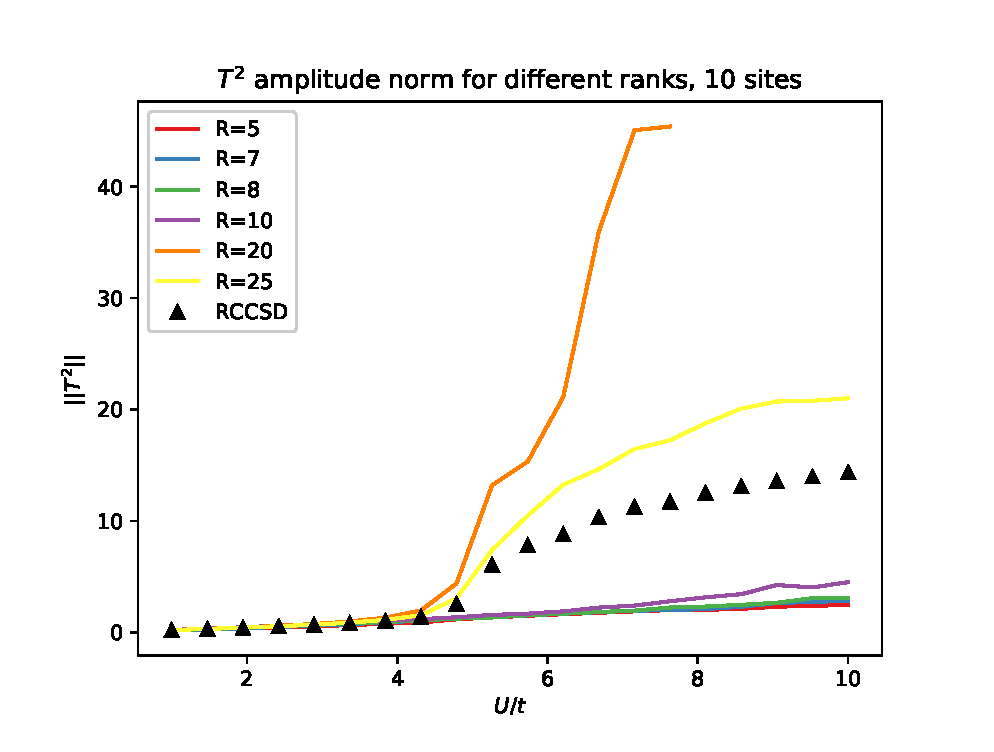
\includegraphics[width=0.9\textwidth]{figures/t2_norms_vs_u_10_sites.eps}
\end{figure}


Finally, let us look at the norms of individual components of $T^{2}$ amplitudes, 
as we keep them in the normalized form (RCCSD-nCPD). The first component 
follows closely the total norm of amplitudes.

\begin{figure}[!htb]
\centering
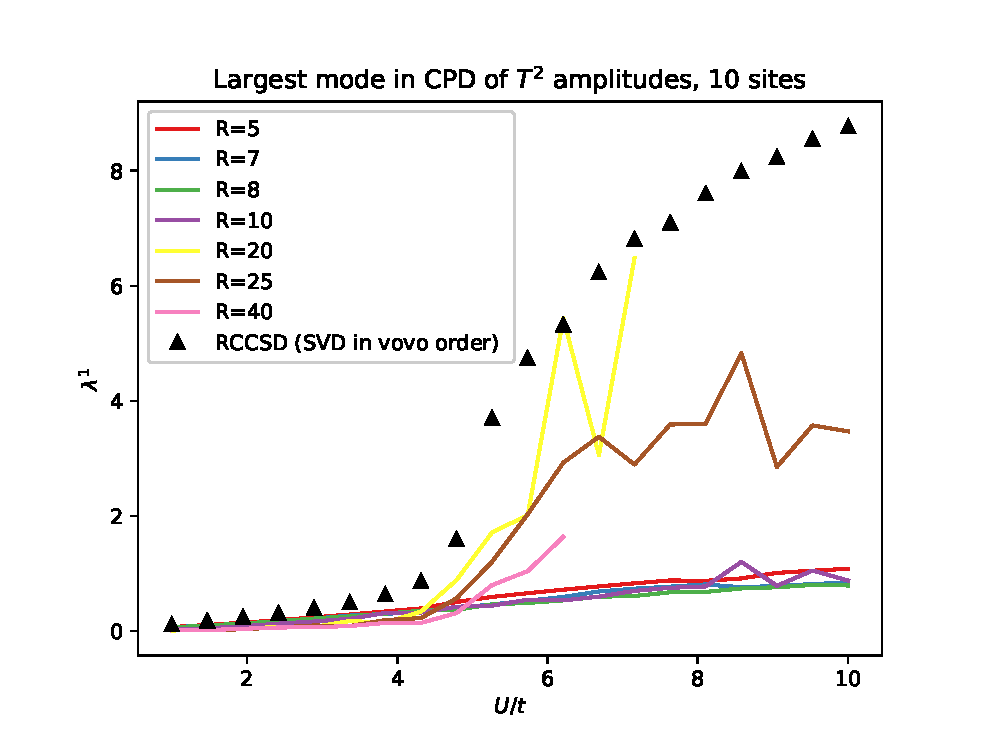
\includegraphics[width=0.9\textwidth]{figures/lam1_vs_u_10_sites.eps}
\end{figure}

The full spectrum, however, does not have a distinct dominant mode
neither in low nor in large rank regime. This contrasts with the case of SVD in 
regular Coupled Cluster, where the broken symmetry mode is clearly seen.
For CPD this is not the case, possibly because the individual 
components of CPD are not orthogonal to each other. Solving this issue (by imposing some 
additional constraint on the structure of $T^2$) will provide a direct way to 
Attenuated CC with decomposed amplitudes.

\begin{figure}[!htb]
\centering
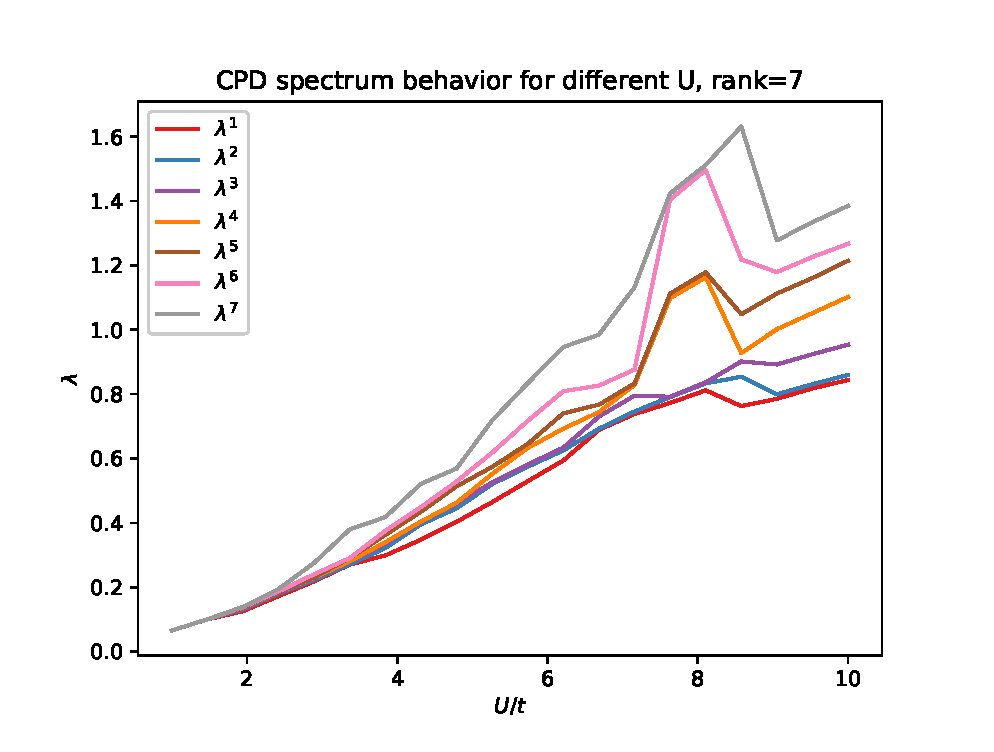
\includegraphics[width=0.9\textwidth]{figures/lam1_lamN_vs_u_10_sites_rank_7.eps}
\end{figure}

\begin{figure}[!htb]
\centering
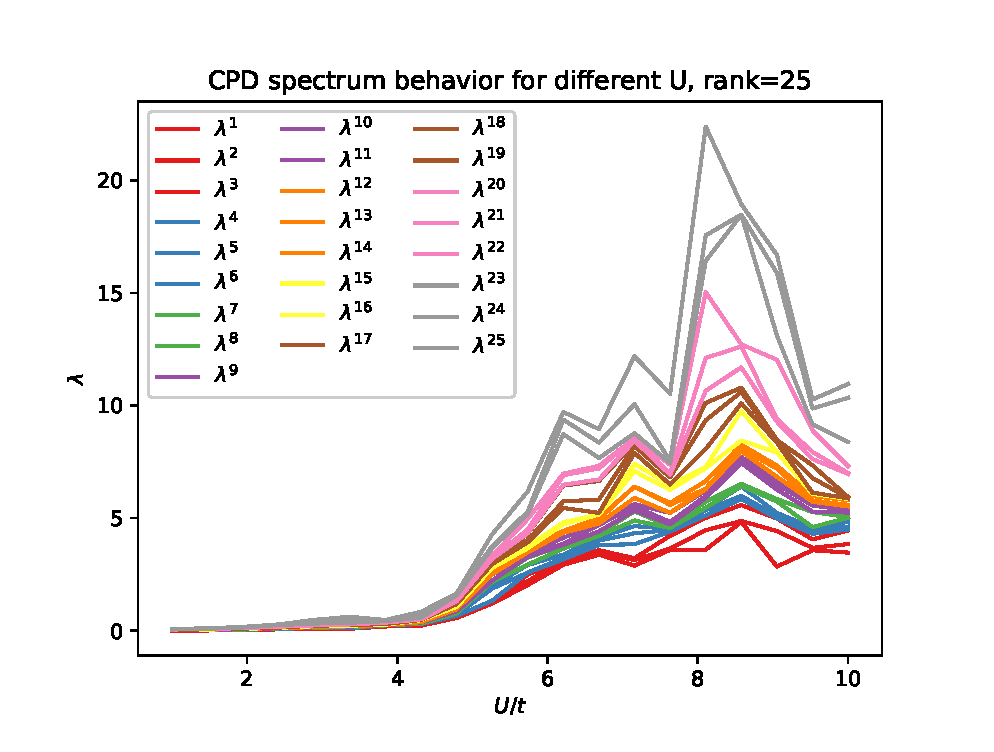
\includegraphics[width=0.9\textwidth]{figures/lam1_lamN_vs_u_10_sites_rank_25.eps}
\end{figure}

\begin{figure}[!htb]
\centering
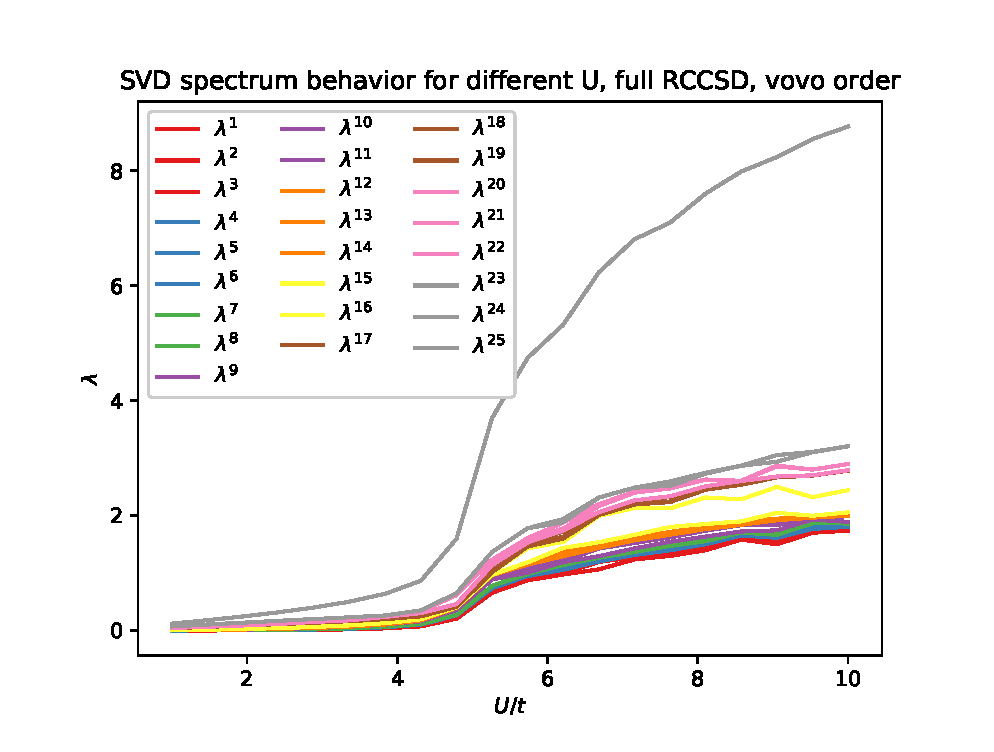
\includegraphics[width=0.9\textwidth]{figures/lam1_lamN_vs_u_10_sites_rccsd_vovo.eps}
\end{figure}

\begin{figure}[!htb]
\centering
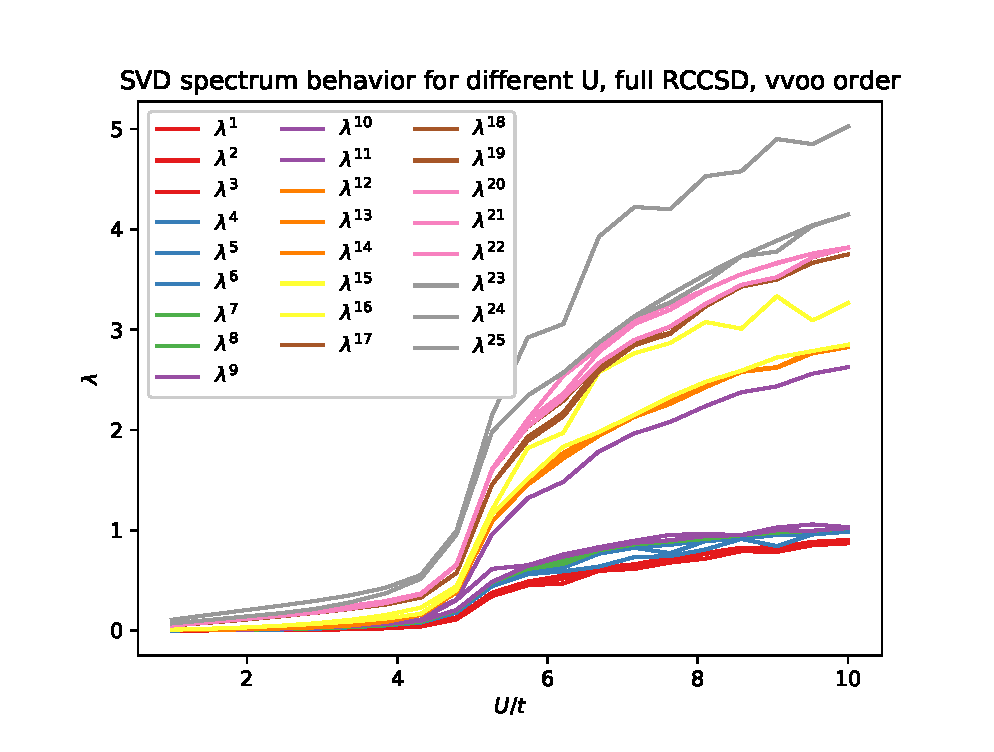
\includegraphics[width=0.9\textwidth]{figures/lam1_lamN_vs_u_10_sites_rccsd_vvoo.eps}
\end{figure}


\end{document}